

\tikzset{every picture/.style={line width=0.75pt}} %set default line width to 0.75pt        
\begin{center}
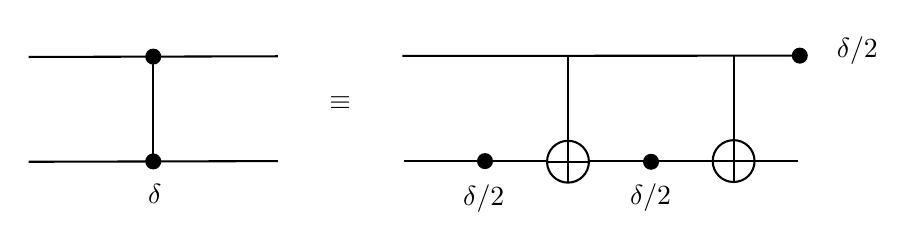
\begin{tikzpicture}[x=0.75pt,y=0.75pt,yscale=-1,xscale=1]
%uncomment if require: \path (0,300); %set diagram left start at 0, and has height of 300

%Straight Lines [id:da21074801917912667] 
\draw    (130.5,140.5) -- (250.5,140.17) ;


%Straight Lines [id:da9874287036079263] 
\draw    (190.5,140.33) -- (190.5,190.83) ;
\draw [shift={(190.5,190.83)}, rotate = 90] [color={rgb, 255:red, 0; green, 0; blue, 0 }  ][fill={rgb, 255:red, 0; green, 0; blue, 0 }  ][line width=0.75]      (0, 0) circle [x radius= 3.35, y radius= 3.35]   ;
\draw [shift={(190.5,140.33)}, rotate = 90] [color={rgb, 255:red, 0; green, 0; blue, 0 }  ][fill={rgb, 255:red, 0; green, 0; blue, 0 }  ][line width=0.75]      (0, 0) circle [x radius= 3.35, y radius= 3.35]   ;
%Straight Lines [id:da4830080618133892] 
\draw    (130.5,191) -- (250.5,190.67) ;


%Straight Lines [id:da1548073386756772] 
\draw    (310.5,140) -- (502,139.86) ;
\draw [shift={(502,139.86)}, rotate = 359.96] [color={rgb, 255:red, 0; green, 0; blue, 0 }  ][fill={rgb, 255:red, 0; green, 0; blue, 0 }  ][line width=0.75]      (0, 0) circle [x radius= 3.35, y radius= 3.35]   ;

%Straight Lines [id:da4883105543582402] 
\draw    (390.32,140.45) -- (390.32,190.95) ;


%Straight Lines [id:da26794551989187454] 
\draw    (311.17,190.67) -- (501.17,190.67) ;


%Straight Lines [id:da5454348469497672] 
\draw    (470.13,140.17) -- (470.13,190.67) ;


%Flowchart: Or [id:dp42872792207775023] 
\draw  [fill={rgb, 255:red, 255; green, 255; blue, 255 }  ,fill opacity=1 ] (380.23,190.95) .. controls (380.23,185.38) and (384.75,180.87) .. (390.32,180.87) .. controls (395.88,180.87) and (400.4,185.38) .. (400.4,190.95) .. controls (400.4,196.52) and (395.88,201.04) .. (390.32,201.04) .. controls (384.75,201.04) and (380.23,196.52) .. (380.23,190.95) -- cycle ; \draw   (380.23,190.95) -- (400.4,190.95) ; \draw   (390.32,180.87) -- (390.32,201.04) ;
%Flowchart: Or [id:dp5893976293181182] 
\draw  [fill={rgb, 255:red, 255; green, 255; blue, 255 }  ,fill opacity=1 ] (460.04,190.67) .. controls (460.04,185.1) and (464.56,180.58) .. (470.13,180.58) .. controls (475.69,180.58) and (480.21,185.1) .. (480.21,190.67) .. controls (480.21,196.24) and (475.69,200.75) .. (470.13,200.75) .. controls (464.56,200.75) and (460.04,196.24) .. (460.04,190.67) -- cycle ; \draw   (460.04,190.67) -- (480.21,190.67) ; \draw   (470.13,180.58) -- (470.13,200.75) ;
%Straight Lines [id:da11444548058172366] 
\draw    (350.33,190.67) ;

\draw [shift={(350.33,190.67)}, rotate = 0] [color={rgb, 255:red, 0; green, 0; blue, 0 }  ][fill={rgb, 255:red, 0; green, 0; blue, 0 }  ][line width=0.75]      (0, 0) circle [x radius= 3.35, y radius= 3.35]   ;
%Straight Lines [id:da1098753753593309] 
\draw    (430.33,191) ;

\draw [shift={(430.33,191)}, rotate = 0] [color={rgb, 255:red, 0; green, 0; blue, 0 }  ][fill={rgb, 255:red, 0; green, 0; blue, 0 }  ][line width=0.75]      (0, 0) circle [x radius= 3.35, y radius= 3.35]   ;

% Text Node
\draw (191.3,206.5) node   {$\delta $};
% Text Node
\draw (349.7,208.5) node   {$\delta /2$};
% Text Node
\draw (280.5,162.5) node   {$\equiv $};
% Text Node
\draw (430.1,208.3) node   {$\delta /2$};
% Text Node
\draw (529.7,137.5) node   {$\delta /2$};


\end{tikzpicture}
\end{center}